\documentclass[preprint]{elsarticle}

\usepackage{lineno,hyperref}
\modulolinenumbers[5]


\usepackage{physics}
\usepackage{graphicx,amsmath,amssymb,mathtools,hyperref,amsfonts,pgfplots,caption,epstopdf,todonotes,tikz,subcaption,geometry}
\usepackage{siunitx}
\usepackage[version=4]{mhchem}
\usepackage{booktabs}

\usetikzlibrary{patterns}
\usetikzlibrary{arrows}
\pgfplotsset{compat=1.13}

\newcommand{\tino}[1]{\todo[inline,color=red!40]{Tino: #1}}
\newcommand{\scott}[1]{\todo[inline,color=green!40]{Scott: #1}}

\geometry{margin=3cm}

\journal{Journal of Power Sources}

%%%%%%%%%%%%%%%%%%%%%%%
%% Elsevier bibliography styles
%%%%%%%%%%%%%%%%%%%%%%%
%% To change the style, put a % in front of the second line of the current style and
%% remove the % from the second line of the style you would like to use.
%%%%%%%%%%%%%%%%%%%%%%%

%% Numbered
%\bibliographystyle{model1-num-names}

%% Numbered without titles
%\bibliographystyle{model1a-num-names}

%% Harvard
%\bibliographystyle{model2-names.bst}\biboptions{authoryear}

%% Vancouver numbered
%\usepackage{numcompress}\bibliographystyle{model3-num-names}

%% Vancouver name/year
%\usepackage{numcompress}\bibliographystyle{model4-names}\biboptions{authoryear}

%% APA style
%\bibliographystyle{model5-names}\biboptions{authoryear}

%% AMA style
%\usepackage{numcompress}\bibliographystyle{model6-num-names}

%% `Elsevier LaTeX' style
\bibliographystyle{elsarticle-num}
%%%%%%%%%%%%%%%%%%%%%%%

%% Put any plot commands in here 

% noniso{D, nx, ylim} 

%\definecolor{c1}{RGB}{102,194,165}
%\definecolor{c2}{RGB}{252,141,98}
%\definecolor{c3}{RGB}{141,160,203}
%\definecolor{c4}{RGB}{231,138,195}
%\definecolor{c5}{RGB}{166,216,84}
%\definecolor{c6}{RGB}{255,217,47}

\definecolor{c1}{RGB}{228,26,28}
\definecolor{c2}{RGB}{55,126,184}
\definecolor{c3}{RGB}{77,175,74}
\definecolor{c4}{RGB}{152,78,163}
\definecolor{c5}{RGB}{255,127,0}
\definecolor{c6}{RGB}{106,61,154}


\pgfplotscreateplotcyclelist{mylist}{
{c1,thick}, 
{c2,thick},
{c3,thick},
{c4,thick},
{c5,thick},
{c1,dashed,thick},
{c1,dotted,thick},
{c2,dashed,thick},
{c2,dotted,thick},
{c3,dashed,thick},
{c3,dotted,thick},
{c4,dashed,thick},
{c4,dotted,thick},
{c5,dashed,thick},
{c5,dotted,thick}}

\newenvironment{customlegend}[1][]{%
    \begingroup
    % inits/clears the lists (which might be populated from previous
    % axes):
    \csname pgfplots@init@cleared@structures\endcsname
    \pgfplotsset{#1}%
}{%
    % draws the legend:
    \csname pgfplots@createlegend\endcsname
    \endgroup
}%

% makes \addlegendimage available (typically only available within an
% axis environment):
\def\addlegendimage{\csname pgfplots@addlegendimage\endcsname}


\newcommand{\LiBattery}{
	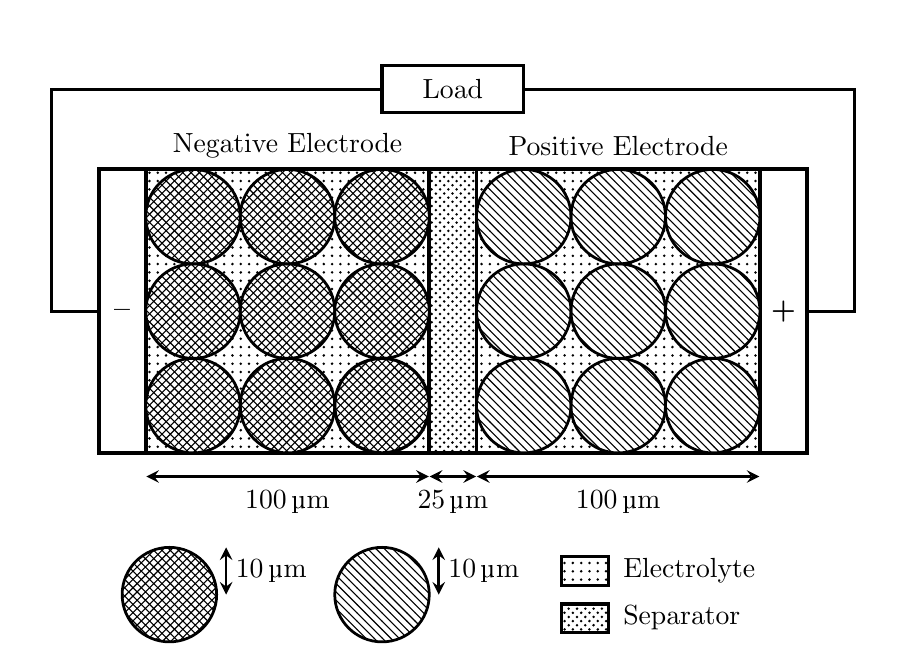
\begin{tikzpicture}[scale=0.6,>=stealth]
    	
        \draw[line width=0.4mm] (-7.5,0) -- (-8.5,0) --(-8.5,4.7)-- (8.5,4.7) -- (8.5,0) -- (7.5,0);
         \draw[line width=0.4mm, fill=white] (-1.5,4.2) rectangle (1.5,5.2);
         \node at (0,4.7){Load};
    	
		\draw[step=1cm,gray,very thin, draw=none] (-9,-7) grid (9,6);
        
        % Electrolyte
        \draw[line width=0.5mm, pattern=dots] (-6.5,-3) rectangle (6.5,3);
        
        % separator
        \draw[fill=white]  (-0.5,-3) rectangle (0.5,3);
        \draw[line width=0.5mm,pattern=crosshatch dots]  (-0.5,-3) rectangle (0.5,3);
        
        % Negative Current Collector
        \draw[line width=0.5mm] (-7.5,-3) rectangle (-6.5,3);
        
        % Positive Current Collector
        \draw[line width=0.5mm] (6.5,-3) rectangle (7.5,3);
        
        % negative electrode       
        \draw[fill=white,draw=none] (-5.5, 2) circle (1cm);
        \draw[fill=white,draw=none] (-5.5, 0) circle (1cm);
        \draw[fill=white,draw=none] (-5.5, -2) circle (1cm);        
        
        \draw[fill=white,draw=none] (-3.5, 2) circle (1cm);
        \draw[fill=white,draw=none] (-3.5, 0) circle (1cm);
        \draw[fill=white,draw=none] (-3.5, -2) circle (1cm);       
        
        \draw[fill=white,draw=none] (-1.5, 2) circle (1cm);
        \draw[fill=white,draw=none] (-1.5, 0) circle (1cm);
        \draw[fill=white,draw=none] (-1.5, -2) circle (1cm);
        
        
        
        \draw[line width=0.35mm,pattern=crosshatch, pattern color = black] (-5.5, 2) circle (1cm);
        \draw[line width=0.35mm,pattern=crosshatch, pattern color=black] (-5.5, 0) circle (1cm);
        \draw[line width=0.35mm,pattern=crosshatch, pattern color=black] (-5.5, -2) circle (1cm);        
        
        \draw[line width=0.35mm,pattern=crosshatch, pattern color=black] (-3.5, 2) circle (1cm);
        \draw[line width=0.35mm,pattern=crosshatch, pattern color=black] (-3.5, 0) circle (1cm);
        \draw[line width=0.35mm, pattern=crosshatch, pattern color=black] (-3.5, -2) circle (1cm);       
        
        \draw[ line width=0.35mm,pattern=crosshatch, pattern color=black] (-1.5, 2) circle (1cm);
        \draw[ line width=0.35mm,pattern=crosshatch, pattern color=black] (-1.5, 0) circle (1cm);
        \draw[ line width=0.4mm,pattern=crosshatch, pattern color=black] (-1.5, -2) circle (1cm);
        
        % positive electrode
        \draw[fill=white,draw=none] (1.5,2) circle (1cm);
        \draw[fill=white,draw=none] (1.5,0) circle (1cm);
        \draw[fill=white,draw=none] (1.5,-2) circle (1cm);
        
        \draw[fill=white,draw=none] (3.5,2) circle (1cm);
        \draw[fill=white,draw=none] (3.5,0) circle (1cm);
        \draw[fill=white,draw=none] (3.5,-2) circle (1cm);
        
        \draw[fill=white,draw=none] (5.5,2) circle (1cm);
        \draw[fill=white,draw=none] (5.5,0) circle (1cm);
        \draw[fill=white,draw=none] (5.5,-2) circle (1cm);
        
		\draw[line width=0.35mm,pattern=north west lines] (1.5,2) circle (1cm);
        \draw[line width=0.35mm,pattern=north west lines] (1.5,0) circle (1cm);
        \draw[line width=0.35mm,pattern=north west lines] (1.5,-2) circle (1cm);
        
        \draw[line width=0.35mm,pattern=north west lines] (3.5,2) circle (1cm);
        \draw[line width=0.35mm,pattern=north west lines] (3.5,0) circle (1cm);
        \draw[line width=0.35mm,pattern=north west lines] (3.5,-2) circle (1cm);
        
        \draw[line width=0.35mm,pattern=north west lines] (5.5,2) circle (1cm);
        \draw[line width=0.35mm,pattern=north west lines] (5.5,0) circle (1cm);
        \draw[line width=0.35mm,pattern=north west lines] (5.5,-2) circle (1cm);
      	
        % Sizes 
        %\draw[line width=0.35mm,<->] (-7.5,-3.5) -- (-6.51,-3.5);
        %\node[below] at (-7,-3.6) {$\SI{25}{\micro\metre}$};
        
        \draw[line width=0.35mm,<->] (-6.49,-3.5) -- (-0.51,-3.5);
        \node[below] at (-3.5,-3.6) {$\SI{100}{\micro\metre}$};
        
        \draw[line width=0.35mm,<->] (-0.49,-3.5) -- (0.49,-3.5);
        \node[below] at (0,-3.6) {$\SI{25}{\micro\metre}$};
        
        \draw[line width=0.35mm,<->] (0.51,-3.5) -- (6.49,-3.5);
        \node[below] at (3.5,-3.6) {$\SI{100}{\micro\metre}$};
        
        %\draw[line width=0.35mm,<->] (6.51,-3.5) -- (7.5,-3.5);
        %\node[below] at (7,-3.6) {$\SI{25}{\micro\metre}$};
        
        %% Bottom Box
        
        %\draw[line width=0.4mm] (-7.5,-7.2) rectangle (7.5,-4.8);
        
        \draw[line width=0.35mm,pattern=crosshatch, pattern color = black] (-6, -6) circle (1cm);
        \draw[line width=0.35mm,<->] (-4.8,-6) -- (-4.8,-5);
        \node[right] at (-4.8,-5.5){$\SI{10}{\micro\metre}$};
        
         \draw[line width=0.35mm,pattern=north west lines, pattern color = black] (-1.5, -6) circle (1cm);
        \draw[line width=0.35mm,<->] (-0.3,-6) -- (-0.3,-5);
        \node[right] at (-0.3,-5.5){$\SI{10}{\micro\metre}$};
              
        
        \draw[line width=0.35mm, pattern=dots] (2.3,-5.8) rectangle (3.3,-5.2);
        \node[right] at (3.4,-5.5){Electrolyte};
        
        \draw[line width=0.4mm, pattern=crosshatch dots] (2.3,-6.8) rectangle (3.3,-6.2);
        \node[right] at (3.4,-6.5){Separator};
        
         % Labels
        \node at (-7,0){{\bf --}};
        \node at (-3.5,3.5){Negative Electrode};
        \node at (3.5,3.5){Positive Electrode};
        
        %\node at (0,3.5){Separator};
        
        \node at (7,0){{\bf +}};
        
	\end{tikzpicture}
}

\newcommand{\voltage}{
	\centering
	\begin{tikzpicture}
	
			\begin{axis}
				[
				width=\textwidth,
				height=0.6\textwidth,
				xlabel={Discharge Capacity ($\SI{}{\ampere\hour/\metre^2}$)},
				ylabel={Voltage (V)},
				xmin=0,
  				xmax=25,
  				ymin=3.2,
  				ymax=3.9,  	
  				minor tick num=1,
  				grid=major, %both, major or minor
  				major grid style={dashed, line width=.1pt},
  				cycle list name=mylist, 
  				legend pos=outer north east,
  				legend style={name=leg}
				]	
				\foreach \x in {0.1, 0.5, 1, 2, 3}{
					\addplot table [col sep=comma, x index=0, y index=1]
					{plot/C\x.dat};
					
					\edef\temp{\noexpand\addlegendentry{\x C}}
					\temp
				}
				\foreach \x in {0.1, 0.5, 1, 2, 3}{
					\addplot table [col sep=comma, x index=0, y index=2]
					{plot/C\x.dat};
					\addplot table [col sep=comma, x index=0, y index=3]
					{plot/C\x.dat};
					}
			\end{axis}
							
			%\node[fill=white, draw, align=center, below=1mm, anchor=north east] (1) at (leg.south east) {Word: Text};
			
			\begin{customlegend}[legend entries={DFN,SPM,SPMe},legend style={at={(leg.south)},below=1mm, anchor=north}]
    			\addlegendimage{black, thick}
    			\addlegendimage{black,dashed, thick}
    			\addlegendimage{black, dotted, thick}
    		\end{customlegend}
	
	\end{tikzpicture}
}


\newcommand{\transient}{
	\begin{center} 
	\begin{tikzpicture}
	
			\begin{axis}
				[
				width=0.9\textwidth,
				height=0.5\textheight,
				xlabel={Discharge Capacity ($\SI{}{\ampere\hour/\metre^2}$)},
				ylabel={Voltage (V)},
				xmin=0,
  				xmax=1.5,
  				ymin=3.72,
  				ymax=3.78,  	
  				minor tick num=1,
  				grid=major, %both, major or minor
  				major grid style={dashed, line width=.1pt},
  				legend pos=north east,
  				legend style={name=leg}
				]	
				{
				\addplot[c1,thick] table [col sep=comma, x index=0, y index=1]
					{plot/voltage/transient1C.dat};
				\addplot[c2,thick, dashed] table [col sep=comma, x index=0, y index=2]
					{plot/voltage/transient1C.dat};
				\addplot[c3,thick, dashed] table [col sep=comma, x index=0, y index=3]
					{plot/voltage/transient1C.dat};
					
					\edef\temp{\noexpand\addlegendentry{DFN}}
					\temp
					\edef\temp{\noexpand\addlegendentry{SPMe}}
					\temp
					\edef\temp{\noexpand\addlegendentry{SPMeT}}
					\temp
				}
			\end{axis}						
	
	\end{tikzpicture}
	\end{center} 
}

\newcommand{\fastDischarge}{
	\begin{center} 
	\begin{tikzpicture}
	
			\begin{semilogyaxis}
				[
				width=0.8\textwidth,
				height=0.8\textheight,
				xlabel={$\hat{\lambda}$},
				ylabel={},
				xmin=1,
  				xmax=70,
  				ymin=1e-12,
  				ymax=1,  	
  				minor tick num=1,
  				grid=major, %both, major or minor
  				major grid style={dashed, line width=.1pt},
  				legend pos=north east,
  				legend style={name=leg}
				]	
				{
				\addplot[c1,thick] table [col sep=comma, x index=0, y index=1]
					{plot/SEI/fastDischargeLiError.csv};
				\addplot[c2,thick, dashed] table [col sep=comma, x index=0, y index=2]{plot/SEI/fastDischargeLiError.csv};
				\addplot[c3,thick] table [col sep=comma, x index=0, y index=1]{plot/SEI/fastDischargeGrowthError.csv};
				\addplot[c5,thick, dashed] table [col sep=comma, x index=0, y index=2]{plot/SEI/fastDischargeGrowthError.csv};
					
					\edef\temp{\noexpand\addlegendentry{Abs($\Delta q^+$)}}
					\temp
					\edef\temp{\noexpand\addlegendentry{$\exp(-\lambda y_0)$}}
					\temp
					\edef\temp{\noexpand\addlegendentry{Abs($\Delta q^-$)}}
					\temp
					\edef\temp{\noexpand\addlegendentry{$\exp(-2\lambda y_0)$}}
					\temp
				}
			\end{semilogyaxis}						
	
	\end{tikzpicture}
	\end{center} 
}

\newcommand{\fastCharge}{
	\begin{center} 
	\begin{tikzpicture}
	
			\begin{axis}
				[
				width=0.8\textwidth,
				height=0.8\textheight,
				xlabel={$\hat{\lambda}$},
				ylabel={Growth rate ($q^-$)}, 
				xmin=0,
  				xmax=200,
  				ymin=-5,
  				ymax=300,  	
  				minor tick num=1,
  				grid=major, %both, major or minor
  				major grid style={dashed, line width=.1pt},
  				legend pos=north west,
  				legend style={name=leg}
				]	
				{
				\addplot[c1,thick] table [col sep=comma, x index=0, y index=1]
					{plot/SEI/fastCharge.csv};
				\addplot[c2,thick, dashed] table [col sep=comma, x index=0, y index=2]{plot/SEI/fastCharge.csv};
					
					\edef\temp{\noexpand\addlegendentry{Numerical}}
					\temp
					\edef\temp{\noexpand\addlegendentry{Analytical}}
					\temp
				}
			\end{axis}						
	\end{tikzpicture}
	\end{center} 
}


 % for tikz and pgfplots code (this just keeps things in the main file clean)

\begin{document}

\begin{frontmatter}


\title{Asymptotic Reduction of Lithium-ion Battery Models}
%\title{Elsevier \LaTeX\ template\tnoteref{mytitlenote}}
\tnotetext[mytitlenote]{Fully documented templates are available in the elsarticle package on \href{http://www.ctan.org/tex-archive/macros/latex/contrib/elsarticle}{CTAN}.}

%% Group authors per affiliation:
\author{Scott Marquis\fnref{oxford}, Valentin Sulzer\fnref{oxford}, Jon Chapman, Colin Please}
\address{University of Oxford}
\fntext[oxford]{Oxford}

%% or include affiliations in footnotes:
\author[mymainaddress,mysecondaryaddress]{Elsevier Inc}
\ead[url]{www.elsevier.com}

\author[mysecondaryaddress]{Global Customer Service\corref{mycorrespondingauthor}}
\cortext[mycorrespondingauthor]{Corresponding author}
\ead{support@elsevier.com}

\address[mymainaddress]{1600 John F Kennedy Boulevard, Philadelphia}
\address[mysecondaryaddress]{360 Park Avenue South, New York}

\begin{abstract}
This template helps you to create a properly formatted \LaTeX\ manuscript.
\end{abstract}

\begin{keyword}
\texttt{elsarticle.cls}\sep \LaTeX\sep Elsevier \sep template
\MSC[2010] 00-01\sep  99-00
\end{keyword}

\end{frontmatter}

\linenumbers

\section{Introduction} 
\subsection{Background}
Lithium-ion batteries are used extensively in consumer electronics and industry. Mathematical models are an essential tool for the design and management of battery systems. The standard mathematical model of a lithium-ion battery is the Doyle-Fuller Newman (DFN) model, which was developed by John Newman and collaborators \cite{doyle,Fuller1994,newman_book}. This model consists of a set of highly coupled nonlinear parabolic and elliptic partial differential equations (PDEs), which must be solved by employing sophisticated numerical techniques. For many applications, the complicated DFN model is not practical and so  simpler models such as the Single Particle Model (SPM) are used instead \cite{Moura2017} (and others). There have been several previous attempts to derive the SPM and corrections to it (ciiite). However, these approaches generally rely on a number of unnecessary assumptions. In this work, we provide a rigorous mathematical derivation of the SPM and an additional correction for the electrolyte by employing asymptotic methods. Similar methods have been used in the derivation of reduced models of lead acid batteries \cite{tino}. With our approach, we require only two assumptions: fast electrical conductivity in the negative and positive electrodes, and fast diffusion in the electrolyte. The validity of both of these assumptions is determined directly from the input parameter values. In comparison, six assumptions that can only be validated by comparison with the full DFN model are required in \cite{Moura2017}. Furthermore, our approach provides information regarding the accuracy of the reduced models. A key result of our work is an electrolyte correction term which predicts the terminal voltage to a higher degree of accuracy than the SPM but with negligible additional computational requirements. 

\subsection{How a Lithium-ion Battery Works}
Lithium-ion batteries consist of two electrodes, a porous separator, an electrolyte, and two current collectors, as displayed in Figure \ref{fig:liBat}. Each electrode consists of active material particles within which lithium can be stored, and a binder which holds the electrode together and maintains electrical conductivity between the active material particles. In Figure \ref{fig:liBat}, we do not display the binder material. 
\begin{figure}[h!]
	\centering
	\LiBattery
    \caption{Schematic of a lithium-ion battery. Active material particles are shaded cross-stitch and diagonally for the negative and positive active materials, respectively.}\label{fig:liBat}
\end{figure} 
Upon discharge, lithium intercalated in the negative electrode particles diffuses to the surface of the particles where a chemical reaction occurs. This chemical reaction produces a lithium ion free to move through the electrolyte and an electron free to move through the electrode. The electron travels through the electrode, into the current collector, through an external wire, and towards the positive electrode. Meanwhile, the lithium ion migrates through the electrolyte towards the positive electrode. At the surface of the positive electrode particles, the lithium ion and the electron combine through another chemical reaction to form a lithium atom intercalated in the positive electrode particle. To charge, a voltage is applied across the cell and the whole process occurs in reverse.

\section{Doyle-Fuller-Newman (DFN) Model}
We summarize here the 1+1D DFN model which is the standard model of a lithium-ion battery \cite{doyle,Fuller1994,newman_book}. The model is derived either by volume averaging \cite{newman_book} or the method of multiple scales \cite{Richardson2011}. Throughout, we use a superscript $*$ to indicate dimensional quantities. As indicated in Figure \ref{fig:liBat}, the thicknesses of the negative electrode, separator, and positive electrode are $L^*_n$, $L_s^*$, and $L_p^*$, respectively. We denote the current collector to current collector thickness of the battery by $L^*=L_n^*+L_s^*+L_p^*$. The active material particles are assumed to be spherically symmetric with radii $R_n$ and $R_p$ in the negative and positive electrodes, respectively. We use the spatial coordinate $x^*\in[0,L^*]$ to indicate the location through the thickness of the battery and the spatial coordinate $r^*\in[0,R_k^*]$ to indicate the location within the active material particles. We define the following regions of the battery
\begin{align*}
    &\Omega^*_n = [0, L_n^*], \\ 
    &\Omega^*_s = [L_n^*, L^*-L_p^*], \\ 
    &\Omega^*_p = [L^*-L_p^*, L^*],
\end{align*}
which correspond to the negative electrode, separator, and positive electrode regions, respectively. We denote electric potentials by $\phi^*$, current densities by $i^*$, and lithium concentrations by $c^*$ (in the electrolyte $c^*$ refers to lithium ion concentrations). To indicate the region within which each variable is defined we include a subscript $k=n,s,p$ which corresponds to $\Omega^*_n$, $\Omega^*_s$, and $\Omega^*_p$, respectively. To distinguish variables in the electrolyte from those in the solid phase of the electrode, we employ an additional subscript $e$ for electrolyte variables. For clarity, the vartiables in the model and their corresponding regions are
\begin{align*}
 & \phi_n^*, \ 
 \phi_{en}^*, \
  c_{en}^*, \
 i_n^*, \
 i_{en}^*: \quad
 &&x^*\in \Omega_{n}^*, \\
 & \phi_{es}^*, \
  c_{es}^*, \
 i_{es}^*: \quad
 &&x^*\in \Omega_{s}^*, 
 \\
  & \phi_p^*, \ 
 \phi_{ep}^*, \
  c_{ep}^*, \
 i_p^*, \
 i_{ep}^*: \quad
 &&x^*\in \Omega_{p}^*, 
 \\
 &c_n^*: &&r^*\in[0,R_n^*],  \quad x^*\in \Omega_{n}^*, 
 \\
 &c_p^*: &&r^*\in[0,R_p^*], \quad x^*\in \Omega_{p}^*.
\end{align*}
We note that $c_n^*$ and $c_p^*$ are dependent on both the macroscopic spatial variable, $x^*$, and the microscopic spatial variable, $r^*$. When stating the governing equations for a variable, we take the region upon which an equation holds to be automatically defined by the subscript, $k=n,s,p$, of the variable. With this in mind, the 1+1D DFN model is summarised as:
\begin{subequations} 
    \begin{align}
        \intertext{Charge Conservation:}
        &\pdv{i_{ek}^*}{x^*} = a_k^* F^* G_k^*,  &&k\in\{n,p\},\\ 
        &\pdv{i_{es}^*}{x^*} = 0, &&\\ 
        &\pdv{i_k^*}{x^*} = -a_k^* F^* G_k^*, &&k\in\{n,p\}, \\
        &i_{ek}^* = \epsilon_k^b \kappa_e^*(c_{ek}^*) \left( - \pdv{\phi_{ek}^*}{x^*} + 2(1-t^+)\frac{R^*T^*}{F^*} \pdv{x^*}\left(\log(c_{ek}^*)\right)\right), && k\in\{n,s,p\}, \\ 
        &i_{k}^* = -\kappa_k^* \pdv{\phi_k^*}{x^*}, && k\in\{n,p\}
        \intertext{Molar Conservation:}
        &\epsilon_k \pdv{c_{ek}^*}{t^*} = \pdv{x^*}\left(\epsilon_k^b D_e^*(c_{ek}^*) \pdv{c_{ek}^*}{x^*}\right) + a_k^* (1-t^+) G_k^*, && k\in\{n,s,p\}, \\ 
        &\pdv{c_k^*}{t^*} = \frac{1}{(r^*)^2}\pdv{r^*}\left((r^*)^2 D_k^*\pdv{c_k^*}{r^*}\right), &&k\in\{n,p\}, 
        \intertext{Electrochemical Reactions:}
    	&G_k^* = \frac{m_k^*}{F^*} (c_k^*)^{1/2} (c_{k,\text{max}}^*-c_k^*)^{1/2}(c_{ek}^*)^{1/2} \sinh\left(\frac{F^*\eta^*_k}{2R^*T^*} \right)\big|_{r^*=R_k^*}, && k\in\{n,p\}, \\ 
    	&\eta^*_k = \phi_k^*\big|_{r^*=R_k^*} - \phi_{ek}^* - U_k^*(c_k^*)\big|_{r^*=R_k^*},  &&k\in\{n,p\}.
    \end{align}
\end{subequations}
with the boundary conditions:
\begin{subequations}
    \begin{align}
        \intertext{Current in Electrodes:}
    &\phi^*_{n}\big|_{x^*=0}=\phi^*_{cn}, \quad \phi^*_{p}\big|_{x^*=1}=\phi^*_{cp}, && \\ 
    &i^*_n\big|_{x^*=0} = \mathcal{I}^*, \quad i^*_n\big|_{x^*=L^*_n} = 0, && \label{eqn:dim:current1}\\
    &i^*_p\big|_{x^*=L^*-L^*_p} = 0, \quad i^*_p\big|_{x^*=L^*} = \mathcal{I}^* && \label{eqn:dim:current2}
\intertext{Current in Electrolyte:}
&i^*_{en,1}\big|_{x^*=0} = 0, \quad i^*_{ep,1}\big|_{x^*=L^*}=0,  && \\ &\phi^*_{en}\big|_{x^*=L^*_n}=\phi_{es}^*\big|_{x^*=L^*_n}, \quad i^*_{en,1}\big|_{x^*=L^*_n}=i^*_{es,1}\big|_{x^*=L^*_n}, && \\ 
&\phi^*_{es}\big|_{x^*=L^*-L^*_p}=\phi^*_{ep}\big|_{x^*=L^*-L^*_p}, \quad 
i^*_{es,1}\big|_{x=L^*-L^*_p}=i^*_{ep,1}\big|_{x^*=L^*-L^*_p}, &&
\intertext{Concentration in Electrolyte:}
&\pdv{c^*_{en}}{x^*}\bigg|_{x^*=0} = 0, \quad \pdv{c^*_{ep}}{x^*}\bigg|_{x^*=L^*}=0,  &&\\ 
&c^*_{en}|_{x^*=L^*_n}=c^*_{es}|_{x^*=L^*_n}, \quad \epsilon_n^b\pdv{c^*_{en}}{x^*}\bigg|_{x^*=L^*_n}=\epsilon_s^b\pdv{c^*_{es}}{x^*}\bigg|_{x^*=L^*_n}, && \\
&c^*_{es}|_{x^*=L^*-L^*_p}=c^*_{ep}|_{x^*=L^*-L^*_p}, \quad \epsilon_s^b\pdv{c^*_{es}}{x^*}\bigg|_{x^*=L^*-L^*_p}=\epsilon_p^b\pdv{c^*_{ep}}{x^*}\bigg|_{x^*=L^*-L^*_p}, && 
\intertext{Concentration in Electrode Active Material:}
&\pdv{c_k^*}{r^*}\bigg|_{r^*=0} = 0, \quad - D^*_k\pdv{c_k^*}{r^*}\bigg|_{r^*=R_k^*} = G_k^*, &&k\in\{n,p\} 
    \end{align}
    
and initial conditions
    \begin{align} 
    	&c_k^*(x^*,r^*,0) = c_{k,0}^*, \quad \phi^*_{k}(x^*,0) = \phi^*_{k,0} , && k\in\{n,p\}\\
        &\phi^*_{ek}(x^*,0) = \phi^*_{e,0}, \quad c_{ek}^*(x^*,0) = c^*_{e,\text{typ}}, && k\in\{n,s,p\}.
    \end{align} 
\end{subequations}

We prescribe the functional forms from Newman's Dualfoil code for $U_n^*(c_n^*)$, $U_p^*(c_p^*)$, and $D_e^*(c_e^*)$, which are the open circuit potentials (OCP) at the negative and positive electrodes and the lithium ion diffusivity in the electrolyte, respectively \cite{newman2004fortran}. A full list of parameters and their values is provided in Table \ref{tab:parameters}. These functions and parameters correspond to a cell with a graphite negative electrode, a \ce{LiPF6} in EC:DMC electrolyte, and a lithium cobalt oxide positive electrode. In (\ref{eqn:dim:current1}) and (\ref{eqn:dim:current2}) $\mathcal{I}^*$ is the actual current density, distinguished from $I^*$ in Table \ref{tab:parameters}, which is the typical current density. We make this distinction to easily accommodate non-constant currents within our reduced models.

\begin{table}[h]
	\centering 
	\resizebox{\textwidth}{!}{%
	\begin{tabular}{c c l c c c} 
	\toprule
     Parameter & Units & Description & $\Omega^*_{n}$ & $\Omega^*_{s}$ & $\Omega^*_{p}$ \\ 
    \midrule 
    $c^*_{e,\text{typ}}$ & $\SI{}{\mol \metre^{-3}}$ & Typical lithium ion concentration in electrolyte & $1\times10^3$ & $1\times10^3$ & $1\times10^3$ \\
    $\tilde{D}_e^*$ & $\SI{}{\metre^{2}/\second}$ & Typical electrolyte diffusivity & $5.34\times10^{-10}$ & $5.34\times10^{-10}$ & $5.34\times10^{-10}$ \\
    $\epsilon_k$ & - & Electrolyte volume fraction & $0.3$ & 1 & $0.3$  \\
    $c^*_{k,\text{max}}$ & $\SI{}{\mol \metre^{-3}}$ & Maximum lithium concentration &$2.4983\times 10^4$ & - & $5.1218\times 10^4$ \\
     $\sigma^*_k$ & $\SI{}{\ohm^{-1}\metre^{-1}}$ & Solid conductivity & 100 & - & 10 \\
     $\tilde{D}^*_k$ & $\SI{}{\metre^{2}/\second}$ & Typical electrode diffusivity &  $3.9\times10^{-14}$ & - &  $1\times10^{-13}$\\
     $R^*_k$ & $\SI{}{\micro\metre}$ & Particle radius & 10 & - & 10  \\
     $a^*_k$ & $\SI{}{\micro\metre^{-1}}$ & Electrode surface area density & 0.18 & - & 0.15 \\
     $m^*_k$ & $\SI{}{\ampere \metre^{-2}(\metre^3/\mol)^{1.5}}$ & Reaction rate & $2\times10^{-5}$ & - & $6\times10^{-7}$ \\
     $L^*_k$ & $\SI{}{\micro\metre}$ & Thickness & 100 & 25 & 100 \\
      \midrule
     $F^*$ & $\SI{}{\coulomb \mol^{-1}}$ & Faraday's constant & & 96487 &  \\
     $R_g^*$ & $\SI{}{\joule \mol^{-1} \kelvin^{-1}}$ & Universal gas constant && 8.314472 & \\
     $T^*$ & $\SI{}{\kelvin}$ & Temperature && 298.15 & \\
     $b$ & - & Bruggeman coefficient && 1.5 &  \\
     $t^+$ & - & Transference number && 0.4 & \\
     $\Phi^*$ &  $\SI{}{V}$ & Typical potential drop across cell & & 1 & \\
     $I^*$ & $\SI{}{A m^{-2}}$ & Typical current density & & 13 & \\
    \bottomrule
	\end{tabular}}
    \caption{Model Parameters: Values taken from Scott Moura's DFN model (based on DUELFOIL parameters).} \label{tab:parameters}
\end{table}


\iffalse
\begin{subequations}
    \begin{align}
        \intertext{Current in Electrodes:}
    &\phi_{n}\big|_{x=0}=\phi_{cn}, \quad \phi_{p}\big|_{x=1}=\phi_{cp}, && \\ 
    &i_n\big|_{x=0} = I, \quad i_n\big|_{x=L_n} = 0, && \\
    &i_p\big|_{x=1-L_p} = 0, \quad i_p\big|_{x=1} = I &&
\intertext{Current in Electrolyte:}
&i_{en,1}\big|_{x=0} = 0, \quad i_{ep,1}\big|_{x=1}=0,  && \\ &\phi_{en}\big|_{x=L_n}=\phi_{es}\big|_{x=L_n}, \quad i_{en,1}\big|_{x=L_n}=i_{es,1}\big|_{x=L_n}, && \\ 
&\phi_{es}\big|_{x=1-L_p}=\phi_{ep}\big|_{x=1-L_p}, \quad 
i_{es,1}\big|_{x=1-L_p}=i_{ep,1}\big|_{x=1-L_p}, &&
\intertext{Concentration in Electrolyte:}
&\pdv{c_{en}}{x}\bigg|_{x=0} = 0, \quad \pdv{c_{ep}}{x}\bigg|_{x=1}=0,  &&\\ 
&c_{en}|_{x=L_n}=c_{es}|_{x=L_n}, \quad \epsilon_n^b\pdv{c_{en}}{x}\bigg|_{x=L_n}=\epsilon_s^b\pdv{c_{es}}{x}\bigg|_{x=L_n}, && \\
&c_{es}|_{x=1-L_p}=c_{ep}|_{x=1-L_p}, \quad \epsilon_s^b\pdv{c_{es}}{x}\bigg|_{x=1-L_p}=\epsilon_p^b\pdv{c_{ep}}{x}\bigg|_{x=1-L_p}, && 
\intertext{Concentration in Electrode Active Material:}
&\pdv{c_k}{r_k}\bigg|_{r_k=0} = 0, \quad -\beta_k\pdv{c_k}{r_k}\bigg|_{r_k=1} = G_k, \quad  && k\in\{n,p\}.
    \end{align}
\end{subequations}
\fi

\iffalse
\begin{table}[h]
	\centering
	\begin{tabular}{|c|c|}\hline
    	Symbol & Description \\ \hline
        $c_e^*$ & Concentration of lithium ions in electrolyte \\ 
        $c_k^*$ & Concentration of lithium in electrode $k=n,p$ \\ 
        $\phi_e^*$ & Electric potential of electrolyte (vs $\ce{Li}$) \\ 
        $\phi_k^*$ & Electric potential of electrode $k=n,p$ (vs $\ce{Li}$) \\ \hline
    \end{tabular}
    \caption{DFN dimensional variables}\label{tab:dimVar}
\end{table} 
\fi

\iffalse
\begin{table}[h]
	\centering 
	\resizebox{\textwidth}{!}{%
	\begin{tabular}{|c|c|c|c|}\hline
  		Symbol & Description & Value & Units \\ \hline
        $\tilde{D}_n^*$ & Typical negative electrode diffusivity & $3.9\times10^{-14}$ & $\SI{}{\metre^{2}/\second}$\\ 
        $\tilde{D}_p^*$ & Typical positive electrode diffusivity & $1\times10^{-13}$ & $\SI{}{\metre^{2}/\second}$ \\ 
        $\kappa_n^*$ & Typical negative electrode conductivity & $100$ & $\SI{}{\ohm^{-1}\metre^{-1}}$ \\ 
        $\kappa_p^*$ & Typical positive electrode conductivity & $10$ & $\SI{}{\ohm^{-1}\metre^{-1}}$ \\ 
        $R_n^*$ & Negative electrode particle radius & $10$ & $\SI{}{\micro\metre}$  \\
        $R_p^*$ & Positive electrode particle radius & $10$ & $\SI{}{\micro\metre}$  \\
        $a_n^*$ & Negative electrode surface area density & $0.18$ & $\SI{}{\micro\metre^{-1}}$ \\ 
        $a_p^*$ & Positive electrode surface area density & $0.15$ & $\SI{}{\micro\metre^{-1}}$ \\ 
        $F^*$ & Faraday's constant & 96487 & \SI{}{\coulomb \mol^{-1}}\\ 
        $m_n^*$ & Negative electrode reaction rate & $2\times 10^{-5}$ & \SI{}{\ampere \metre^{-2} (\metre^3/\mol)^{1.5}} \\
        $m_p^*$ & Positive electrode reaction rate & $6\times 10^{-7}$ & \SI{}{\ampere \metre^{-2} (\metre^3/\mol)^{1.5}}\\
        $c_{n,\text{max}}^*$ & Maximum lithium concentration in negative electrode & $2.4983\times 10^4$ & \SI{}{\mol \metre^{-3}} \\ 
        $c_{p,\text{max}}^*$ & Maximum lithium concentration in positive electrode & $5.1218\times 10^4$ & \SI{}{\mol \metre^{-3}} \\    
        $c_{e,\text{typ}}^*$ & Typical lithium ion concentration in electrolyte & $1\times10^3$ & \SI{}{\mol \metre^{-3}} \\ 
        $R^*$ & Universal gas constant & 8.314472 & \SI{}{\joule \mol^{-1} \kelvin^{-1}}\\
        $T^*$ & Temperature & 298.15 & \SI{}{\kelvin} \\
        $\epsilon_n$ & Electrolyte volume fraction in negative electrode & $0.3$ & -\\
        $\epsilon_{\text{sep}}$ & Electrolyte volume fraction in separator & $1$ & -\\
        $\epsilon_p$ & Electrolyte volume fraction in positive electrode & $0.3$ & -\\
        $\tilde{D}_e^*$ & Typical electrolyte diffusivity & $5.34\times10^{-10}$ & $\SI{}{\metre^{2}/\second}$ \\
        $b$ & Bruggeman coefficient & 1.5 & - \\
        $t^+$ & Transference number & 0.4 & - \\
        $L_n^*$ & Thickness of negative electrode &$100$ & $\SI{}{\micro\metre}$  \\
        $L_{s}^*$ & Thickness of separator &$25$ & $\SI{}{\micro\metre}$ \\
        $L_p^*$ & Thickness of positive electrode &$100$ & $\SI{}{\micro\metre}$  \\ 
        $L^*$ & Thickness of full cell & $225$ & $\SI{}{\micro\metre}$ \\
        $\Phi$ & Typical potential drop across cell & $\SI{1}{V}$ \\
        $I^*$ & Current density & - & $\SI{}{A m^{-2}}$ \\ \hline
    \end{tabular}}
    \caption{Dimensional Parameters: Values taken from Scott Moura's DFN model (based on DUELFOIL parameters)} \label{tab:dimensional}
\end{table}
\fi


\section{Asymptotic Reduction of DFN Model}

\subsection{Dimensionless Form of DFN Model}
We use asymptotic methods to reduce the DFN model to simpler forms. To do this, we first nondimensionalise the DFN model by making the following scalings: 
\begin{gather}	
	\begin{split}
	r^* = R_s^* r_s, \quad x^* = L^* x, \quad t^* = \tau_d^* t \\ 
    c_n^* = c_{n,\text{max}}^*c_n, \quad c_e^* = c_{e,\text{typ}}^* c_e, \quad c_p^* = c_{p,\text{max}}^* c_p, \\
    \phi_n^* = \Phi^* \phi_n, \quad \phi_e^* = \Phi^* \phi_e, \quad \phi_p^*=\Phi^* \phi_p, \\ 
    U_n^*(c_n^*) = \Phi^* U_n(c_n) \quad U_p^*(c_p^*) = \Phi^* U_p(c_p) \\
    i_n^*= J^* i_n, \quad i_e^* = J^* i_e, \quad i_p^* = J^* i_p, \\ 
    G_n^* = \frac{J^*}{a_n^* F^* L^*}G_n, \quad G_p^* = \frac{J^*}{a_p^* F^* L^*}G_p, \\ 
    D_e^*(c_e^*) = \tilde{D}_e^* D_e(c_e) \quad 
    \kappa^*_e(c_e^*) = \frac{(F^*)^2 \tilde{D}_e^* c_{e,\text{typ}}^*}{R^*T^*}\kappa(c_e)
    \end{split}
\end{gather} 
and identify the following timescales in the model: 
\begin{gather} 
	\begin{split}
	\tau_d^*=\frac{F^* c_{n,\text{max}}^* L^*}{J^*},\quad \tau_n^* = \frac{(R_n^*)^2}{D_n^*}, \quad \tau_e^* = \frac{(L^*)^2}{\tilde{D}_e^*}, \\ \tau_p^* = \frac{(R_p^*)^2}{D_p^*}, \quad \tau_{r_n}^* = \frac{F^*}{m_n^* a_n^* (c_{e,\text{typ}}^*)^{1/2}}, \quad \tau_{r_p}^* = \frac{F^*}{m_p^* a_p^* (c_{e,\text{typ}}^*)^{1/2}},
    \end{split}
\end{gather} 
which correspond to the discharge timescale, the negative electrode diffusion timescale, electrolyte diffusion timescale, the positive electrode diffusion timescale, the negative electrode reaction timescale, and the positive electrode reaction timescale, respectively. Here, $J^*$ is a typical discharge current density for the battery introduced to allow our work to be easily extended to time dependent current densities. We then identify the following dimensionless parameters
\begin{gather} 
	\begin{split}
	\gamma_n = \frac{\tau_d^*}{\tau_n^*}, \quad \gamma_p = \frac{\tau_d^*}{\tau_p^*}, \quad \beta_n = a_n^*R_n^*, \quad \beta_p = a_p^*R_p^*, \\ 
    \kappa_n = \frac{\kappa_n^* \Phi^*}{J^* L^*}, \quad \kappa_p = \frac{\kappa_p^* \Phi^*}{J^* L^*}, \quad m_n =\frac{\tau_d^*}{\tau_{r_n}^*}, \quad m_p =\frac{\tau_d^*}{\tau_{r_p}^*}, \\ 
    \hat{C}_k=\frac{c_{k,\text{max}}^*}{c_{n,\text{max}}^*}, \quad \nu=\frac{c_{n,\text{max}}^*}{c_{e,\text{typ}}^*}, \quad \lambda=\frac{F^* \Phi^*}{R^* T^*}, \quad \delta = \frac{\tau_e^*}{\tau_{d}^*}, \quad I=\frac{I^*}{J^*}.
    \end{split}
\end{gather}
The values of these dimensionless parameters corresponding to the values of the dimensional parameters in Table \ref{tab:dimensional} are given in Table \ref{tab:nonDim}. The resulting dimensionless equations are summarized as: 

\begin{subequations}\label{eqn:DFN} 	
	
     \begin{gather} 
    	\delta \epsilon_k \pdv{c_e}{t} = \pdv{x}\left(\epsilon_k^b  D_e(c_e) \pdv{c_e}{x}\right) + \delta \nu (1-t^+) G_k \label{eqn:nDim:electrolyte:concentration}\\
    	\pdv{i_e}{x} = G_k, \label{eqn:nDim:electrolyte:current} \\ 
        \delta \nu i_e = \epsilon_k^b  \kappa(c_e) \left( -\lambda \pdv{\phi_e}{x} + 2(1-t^+) \pdv{x}\left(\log(c_e)\right)\right)\label{eqn:nDim:McIn}
    \end{gather} 
    
	\begin{gather}
     \pdv{c_k}{t} = \gamma_k \frac{1}{r_k^2}\pdv{r_k}\left(r_k^2 \pdv{c_k}{r_k}\right), \label{eqn:nDim:solid:concentration} \\
     \pdv{c_k}{r}\big|_{r_k=0} = 0, \ \ - \beta_k \hat{C}_k \gamma_k  \pdv{c_k}{r_k}\big|_{r_k=1} = G_k \label{eqn:nDim:solid:con:BC} \\
    	\pdv{i_k}{x} = - G_k \label{eqn:nDim:solid:current}\\  
        i_k = - \kappa_k \pdv{\phi_k}{x}, \label{eqn:nDim:solid:ohms}
    \end{gather}    
 
    \begin{align} 
    \begin{split}
    	G_k &= m_k \hat{C}_k c_k^{1/2} (1-c_k)^{1/2}c_e^{1/2} \sinh\left(\frac{\lambda \eta_k}{2} \right)\big|_{r_s=1}, \\ \eta_k &= \phi_k - \phi_e - U_k(c_k) \label{eqn:nDim:BV}
    \end{split}
    \end{align} 
    
with the boundary conditions: 
    
    \begin{gather}\label{eqn:nDim:BC}
    	\pdv{c_e}{x}\big|_{x=0,1}=0, \quad i_e\big|_{x=0,1}=0, \quad i_e\big|_{x=l_n,1-l_p}=I
    \end{gather}     
and initial conditions 
    \begin{gather}\label{eqn:nDim:init}
    	c_k(x,r,0) = c_{k,0}, \ \ c_e(x,0) = 1, \ \ \phi_{e}(x,0) = \phi_{e,0}, \ \ \phi_{s}(x,0) = \phi_{s,0}.
    \end{gather} 
\end{subequations}

\begin{table}[h]
	\centering
	\begin{tabular}{|c|c|}\hline
    	Symbol & Value \\ \hline
        $\gamma_n$ & 8.8136 / $\mathcal{C}$ \\ 
        $\gamma_p$ & 22.5990 / $\mathcal{C}$ \\ 
        $\beta_n$ & 1.8 \\
        $\beta_p$ & 1.5 \\ 
        $\kappa_n$ & $1.8519\times10^4/ \mathcal{C}$  \\ 
        $\kappa_p$ & $1.8519\times10^3/ \mathcal{C}$\\ 
        $m_n$ & $26.6639/ \mathcal{C}$ \\ 
        $m_p$ & $1.3666/ \mathcal{C}$ \\ 
        $\hat{C}_n$ & 1 \\ 
        $\hat{C}_p$ & 2.0501\\
        $\nu$ & 24.9833 \\
        $\lambda$ & 38.9224 \\ 
        $\delta$ & $0.0042 \mathcal{C}$ \\ \hline
    \end{tabular}
    \caption{Derived dimensionless parameters: Here $\mathcal{C}=I^*/24$ is the C-Rate where we have taken a 1C rate to correspond to a current density of \SI{24}{\ampere \metre^{-2}}. This is for a cell with an initial stochoimetry of $0.8$ in the negative electrode and $0.6$ in the positive electrode with a voltage cutoff of \SI{3.2}{\volt}.}\label{tab:nonDim}
\end{table} 

\subsection{Leading Order Model}
A key observation from Table \ref{tab:nonDim} is that for C-rates below 5C, we have that $1/\kappa_k \ll \delta \ll 1$, whereas all other parameters are approximately $\mathcal{O}(1)$. This corresponds to fast conduction of electrons through the solid phase and fast diffusion of lithium-ions in the electrolyte relative to the timescale for lithium diffusion in the electrolyte particles. Therefore, we seek the following asymptotic expansions
\begin{align*} 
	&c_k \sim c_k^0 + \delta c_k^1 + \dots \ \ 
    &&c_k \sim c_k^0 + \delta c_k^1 + \dots \\ 
    &\phi_k \sim \phi_k^0 + \delta \phi_k^1 + \dots \ \ 
    &&\phi_e \sim \phi_e^0 + \delta \phi_e^1 + \dots \\
    &i_k \sim i_k^0 + \delta i_k^1 + \dots \ \ 
    &&i_e \sim i_e^0 + \delta i_e^1 + \dots \\    
     &G_k \sim G_k^0 + \delta G_k^1 + \dots 
\end{align*}
At leading order, (\ref{eqn:nDim:electrolyte:concentration}) gives
\begin{equation}
	\pdv{x}\left(\mathcal{D}_e(c_e^0) \pdv{c_e^0}{x}\right) = 0, 
\end{equation}
which in conjunction with (\ref{eqn:nDim:BC}) determines that $c_e^0$ is independent of $x$. Furthermore, we also have that $c_e^0(x,0)=1$ from (\ref{eqn:nDim:init}). At $\mathcal{O}(\delta)$, (\ref{eqn:nDim:electrolyte:concentration}) is
\begin{equation}\label{eqn:order1:concentration} 
	\pdv{c_e^0}{t} = \pdv{x} \left(\epsilon_k^b D_e(c_e^0)\pdv{c_e^1}{x} \right) + \nu (1-t^+) \pdv{i_e^0}{x},
\end{equation} 
where we have used $G_k^0 = \pdv{i_e^0}{x}$. Integration of (\ref{eqn:order1:concentration}) over $x\in[0,1]$ and application of the boundary conditions (\ref{eqn:nDim:BC}) at leading and first order, gives that $c_e^0$ is time independent. Therefore $c_e^0(x,t)=1$. Equation (\ref{eqn:nDim:McIn}) at leading order, then gives: 
\begin{equation}
	\pdv{\phi_e^0}{x} = 0 
\end{equation}
and so $\phi_e^0(x,t) = \phi_e^0(t)$. We now take advantage of the fact that $1/\kappa_k \ll \delta$, so that at leading order (\ref{eqn:nDim:solid:ohms}) gives 
\begin{equation}
	\pdv{\phi_k^0}{x} = 0 
\end{equation}
and hence $\phi_k^0 = \phi_k^0(t)$.  
Since $c_k^0$ is initially independent of $x$ and $c_e^0$, $\phi_e^0$, and $\phi_k^0$ are all independent of $x$, it follows from (\ref{eqn:nDim:BV}) at leading order that $G_k^0$ and $c_k^0$ are independent of $x$ for all time. Therefore, we can integrate (\ref{eqn:nDim:electrolyte:current}) over electrode $k$ and apply (\ref{eqn:nDim:BC}) to find: 
\begin{gather} 
	i_e^0 = 
    \begin{cases} 
    \frac{x}{l_n}I, &0\leq x \leq l_n \\
    I, & l_n\leq x \leq 1-l_p \\
    \frac{1-x}{l_p}I, & l_p\leq x \leq 1
    \end{cases}
\end{gather} 
which also determines that
\begin{equation} 
	G_n^0=\frac{I}{l_n}, \quad G_p^0=-\frac{I}{l_p}.
\end{equation}
Solving (\ref{eqn:nDim:BV}) at leading order gives
\begin{equation}\label{eqn:lo:phi}
	\phi_k^0 = \phi_e^0 + U_k(c_k^0) + \frac{2}{\lambda}\sinh^{-1}\left( \frac{G_k^0}{g_k^0} \right), \ \ \text{for} \ k\in\{n,p\}, 
\end{equation}
where 
\begin{equation}\label{eqn:gk0} 
g_k^0=m_k \hat{C}_k (c^0_k)^{1/2} (1-c_k^0)^{1/2}(c_e^0)^{1/2}.
\end{equation}
from which we can determine the leading order terminal voltage, $V^0=\phi_p^0-\phi_n^0$, as
\begin{subequations}\label{eqn:SPM} 
\begin{align} 
	\begin{split}
	V^0 = &U_p(c_p^0) - U_n(c_n^0) - \frac{2}{\lambda}\sinh^{-1}\left( \frac{I}{g_p^0 l_p} \right) - \frac{2}{\lambda} \sinh^{-1}\left( \frac{I}{g_n^0 l_n} \right).
    \end{split} 
\end{align} 

Therefore, only $c_k^0$ remains to be determined to obtain the leading order terminal voltage. At leading order (\ref{eqn:nDim:solid:concentration}), (\ref{eqn:nDim:solid:con:BC}), and (\ref{eqn:nDim:init}) give 
	\begin{align} \label{eqn:lo:solidConcentration} 
     \pdv{c_k^0}{t} = \gamma_k \frac{1}{r_k^2}\pdv{r_k}\left(r_k^2 \pdv{c_k^0}{r_k}\right), \\
     \pdv{c_k^0}{r}\big|_{r_k=0} = 0, \ \ - \beta_k\hat{C}_k \gamma_k \pdv{c_k^0}{r_k}\big|_{r_k=1} = G_k^0  \label{eqn:lo:solidConcentration:BC} \\ 
     c_k^0(r,0) = c_{k,0} 
    \end{align} 
\end{subequations} 
which is to be solved numerically. We identify (\ref{eqn:SPM}) as the dimensionless form of the commonly used SPM \cite{Bizeray2017,Perez2016}. \\

\subsection{Next Order Correction}
We now proceed to $\mathcal{O}(\delta)$ to extend the range of applicability of the SPM to higher C-rates. At $\mathcal{O}(\delta)$, (\ref{eqn:nDim:electrolyte:concentration}) becomes
\begin{equation}\label{eqn:od:electrolyte} 
    	 \pdv{x}\left(\epsilon_k^b D_e(c^0_e) \pdv{c^1_e}{x}\right) + \nu (1-t^+) G_k^0 = 0. 
\end{equation} 
The conditions of continuity of flux and concentration of lithium at the electrode--separator boundaries are given as
\begin{align}
	\begin{split}
	c_{e,n}=c_{e,s}, \quad \epsilon_n^b \pdv{c_{e,n}^1}{x} = \epsilon_s^b \pdv{c_{e,s}^1}{x}, \quad \text{on} \, x=l_n, \\
    c_{e,s}=c_{e,p}, \quad \epsilon_s^b \pdv{c_{e,s}^1}{x} = \epsilon_p^b \pdv{c_{e,p}^1}{x}, \quad \text{on} \, x=1-l_p, \label{eqn:continuityConditions}
    \end{split}
\end{align}
where $c_{e,k}$ is the electrolyte concentration in region $k=n,s,p$. We integrate (\ref{eqn:od:electrolyte}) over the entire cell, employ (\ref{eqn:continuityConditions}),  and apply the leading order boundary conditions from (\ref{eqn:nDim:BC}), to find: 
\begin{align} 
	\begin{split}\label{eqn:od:c1}
	c_e^1(x) =&\frac{\nu (1-t^+) I}{ 6 \mathcal{D}(c_e^0)}\left(\rule{0cm}{1cm} 2\left(\frac{l_p^2}{\epsilon_p^b} - \frac{l_n^2}{\epsilon_n^b}\right) \right.\\ &\left. + 3\begin{cases} 
    	  \frac{l_{sep}}{\epsilon_{sep}^b}(1+l_p-l_n) + \frac{1}{\epsilon_n^b l_n}(l_n^2-x^2) , & 0\leq x \leq l_n \\
    	  \frac{1}{\epsilon_{sep}^b}(l_n^2 - l_p^2 + 1-2x) , & l_n\leq x \leq 1-l_p \\
    	  \frac{l_{sep}}{\epsilon_{sep}^b}(l_p - l_n - 1) + \frac{1}{l_p \epsilon_p^b}( (x-1)^2 - l_p^2 ), & 1-l_p\leq x \leq 1
    \end{cases}  \rule{0cm}{1cm}\right). 
    \end{split}
\end{align} 
At $\mathcal{O}(\delta)$, (\ref{eqn:nDim:McIn}) becomes
\begin{gather} 
        \nu i_e^0 = \epsilon_k^b \kappa(c_e^0) \left( -\lambda \pdv{\phi^1_e}{x} + \frac{2(1-t^+)}{c_e^0} \pdv{c_e^1}{x} \right). \label{eqn:mcCin:order1}
\end{gather} 
Integration of (\ref{eqn:mcCin:order1}) with respect to $x$, gives
\begin{equation} 
	\phi_e^1(x) =\tilde{\phi}_e^1 + \frac{2(1-t^+)}{\lambda c_e^0}c_e^1 - \frac{\nu}{\lambda \kappa(c_e^0)}
    \begin{cases} 
    	   \frac{x^2-l_n^2}{2 \epsilon_n^b l_n} + \frac{l_n}{\epsilon_{sep}^b}, & 0\leq x \leq l_n \\
    	   \frac{x}{\epsilon_{sep}^b}, & l_n\leq x \leq 1-l_p \\
    	   \frac{x(2-x)+l_p^2-1}{2\epsilon_p^b l_p} + \frac{1-l_p}{\epsilon_{sep}^b}, & 1-l_p\leq x \leq 1.
    \end{cases}  
\end{equation} 
where $\tilde{\phi}_e^1$ is independent of $x$. At $\mathcal{O}(\delta)$ (\ref{eqn:nDim:electrolyte:current}) and (\ref{eqn:nDim:BC}) become
\begin{subequations} 
\begin{align}
	\pdv{i_e^1}{x} = G_k^1, \label{eqn:od:elect:curr}\\ 
	i_e^1\bigg|_{x=0,l_n,1-l_p,1} = 0. \label{eqn:od:elect:curr:bc}
\end{align} 
\end{subequations}
Integration of (\ref{eqn:od:elect:curr}) over each electrode and applying (\ref{eqn:od:elect:curr:bc}) gives the conditions
\begin{equation}\label{eqn:od:conditions} 
	\int_0^{l_n} G_n^1(x,t)\, \text{d}x = 0, \ \ \int_{1-l_p}^1 G_p^1(x,t)\, \text{d}x = 0. 
\end{equation}
The $\mathcal{O}(\delta)$ component of (\ref{eqn:nDim:BV}) is given by
\begin{subequations} 
    \begin{gather} \label{eqn:od:BV}
    	G_k^1 = \frac{g_k^0}{2} \left( g_k^1 \sinh\left( \frac{\lambda\eta_k^0}{2}  \right) + \cosh(\frac{\lambda\eta_k^0}{2} ) \lambda \eta_k^1 \right)\bigg|_{r_k=1}, \\ \eta_k^0 = \phi^0_k - \phi^0_e - U_s(c_k^0), \ \ \eta_k^1 = \phi^1_k - \phi^1_e - U_k'(c^0_k)c_k^1,\\
    g_k^1 = \left(\frac{c_k^1}{c_k^0} - \frac{c_k^1}{1-c_k^0} + \frac{c_{e,k}^1}{c_e^0} \right), 
    \end{gather} 
\end{subequations} 
where $g_k^0$ is given by (\ref{eqn:gk0}). Given that $1/\kappa_k\ll\delta$, (\ref{eqn:nDim:solid:current}) at $\mathcal{O}(\delta)$ yields $\phi_k^1=\phi_k^1(t)$. We now average (\ref{eqn:od:BV}) over electrode $k$, apply the conditions in (\ref{eqn:od:conditions}), and rearrange for $\phi_k^0$ to find:
\begin{gather}\label{eqn:od:BV_av}
	\phi_k^1 = \bar{\phi}_{e,k}^1 + U_s'(c_k^0)\bar{c}_k^1 - \frac{\bar{g}_k^1G_k^0}{\lambda\sqrt{(g_k^0)^2 + (G_k^0)^2}}, \ \ k\in\{n,p\},
\end{gather} 
where we have used that
\begin{equation} 
	\tanh\left(\sinh^{-1}\left(\frac{G_k^0}{g_k^0} \right) \right) = \frac{G_k^0}{\sqrt{(g_k^0)^2 + (G_k^0)^2}},
\end{equation}
and an overbar indicates the electrode averaged quantities of the form:
\begin{equation*}
	\bar{y}_n = \frac{1}{l_n}\int_{0}^{l_n}y_n\, \text{d}x, \quad 		\bar{y}_p = \frac{1}{l_p}\int_{1-l_p}^{1}y_p\, \text{d}x.
\end{equation*}
Upon calculation, the electrode averaged quantities are given as:
\begin{subequations}  
\begin{align} 	
	\bar{c}_{e,n}^1 &= \frac{\nu (1-t^+) I}{ 6 \mathcal{D}(c_e^0)}\left( 2\left(\frac{l_p^2}{\epsilon_p^b} - \frac{l_n^2}{\epsilon_n^b} \right) + \frac{2 l_n}{\epsilon_n^b} + \frac{3l_{sep}}{\epsilon_{sep}^{b}}(l_p-l_n+1)\right) \\ 
    \bar{c}_{e,p}^1 &= \frac{\nu (1-t^+) I}{ 6 \mathcal{D}(c_e^0)}\left( 2\left(\frac{l_p^2}{\epsilon_p^b} - \frac{l_n^2}{\epsilon_n^b} \right) - \frac{2 l_p}{\epsilon_p^b} + \frac{3l_{sep}}{\epsilon_{sep}^{b}}(l_p-l_n-1)\right) \\ 
    \bar{\phi}_{e,n}^1 &= \tilde{\phi}_e^1 +\frac{2(1-t^+)}{\lambda c_e^0} \bar{c}_{e,n}^1 + \frac{\nu Il_n}{\lambda \kappa(c_e^0)}\left(\frac{1}{3 \epsilon_{n}^b} - \frac{1}{\epsilon_{sep}^b}\right) \\ 
    \bar{\phi}_{e,p}^1 &= \tilde{\phi}_e^1 +\frac{2(1-t^+)}{\lambda c_e^0} \bar{c}_{e,p}^1 + \frac{\nu Il_p}{\lambda \kappa(c_e^0)}\left(\frac{1}{ \epsilon_{sep}^b} - \frac{1}{3\epsilon_p^b}\right) - \frac{\nu I}{\lambda \kappa(c_e^0)\epsilon_{sep}^b} \\
    \bar{g}_k^1 =& \left(\frac{\bar{c}_k^1}{c_k^0} - \frac{\bar{c}_k^1}{1-c_k^0} + \frac{\bar{c}_{e,k}^1}{c_e^0} \right).
\end{align} 
\end{subequations} 
Taking the $O(\delta)$ component of (\ref{eqn:nDim:solid:concentration}), (\ref{eqn:nDim:solid:con:BC}), and (\ref{eqn:nDim:init}) and averaging over electrode $k$ gives the following problem for $\bar{c}_k^1$: 
\begin{gather}
     \pdv{\bar{c}_k^1}{t} = \gamma_k \frac{1}{r_k^2}\pdv{r_k}\left(r_k^2 \pdv{\bar{c}_k^1}{r_s}\right), \\
     \pdv{\bar{c}_s^1}{r}\bigg|_{r_s=0} = 
     \pdv{\bar{c}_s^1}{r_s}\bigg|_{r_s=1} = 0, \\ 
     \bar{c}_k^1(r, 0) = 0.
    \end{gather} 
We then must have ${\bar{c}_k^1(r,t)=0}$ for all time (this also holds for concentration dependent diffusivity). Therefore, our next order correction to the terminal voltage, ${V^1=\phi_p^1-\phi_n^1}$, is given by
\begin{align}\label{eqn:voltageCorrection}
\begin{split} 
V^1 = &-\frac{2 \nu (1-t^+)^2I}{\lambda \mathcal{D}(c_e^0)c_e^0}\left( \frac{l_n}{3 \epsilon_n^b} + \frac{l_{sep}}{\epsilon_{sep}^b} + \frac{l_p}{3\epsilon_p^b} \right) \\ 
    & - \frac{\nu I}{\lambda \kappa(c_e^0)} \left(\frac{l_n}{3\epsilon_n^b} - \frac{l_n - 1 + l_p}{\epsilon_{sep}^b} + \frac{l_p}{3\epsilon_p^b} \right) \\
    &+ \frac{\bar{g}_p^1 I }{\lambda \sqrt{(g_p^0l_p)^2+I^2}} + \frac{\bar{g}_n^1 I }{\lambda \sqrt{(g_n^0l_n)^2+I^2}}.  
\end{split}
\end{align} 
With this algebraic correction term the terminal voltage is given by $V=V^0+\delta V^1$ which is $\mathcal{O}(\delta^2,1/\kappa_p)$ accurate instead of  $\mathcal{O}(\delta)$ accurate in the case of the SPM.

\subsection{Simplified Expression and Model Interpretation} 
In order to simplify the final form of our corrected voltage and aid with interpretation, we note that
\begin{align*} 
	&-\frac{2}{\lambda}\sinh^{-1}\left(\frac{I}{\bar{g}_k l_k}\right) = -\frac{2}{\lambda}\sinh^{-1}\left(\frac{I}{g_k^0l_k} \right)
    +\delta \frac{\bar{g}_k^1 I}{\lambda\sqrt{(g_k^0l_k)^2+I^2}} 
    + \mathcal{O}\left(\delta^2\right)
\end{align*} 
where 
\begin{equation} 
	\bar{g}_k = m_k  (c_k^0)^{1/2}(1-c_k^0)^{1/2}(c_e^0+\delta\bar{c}_{e,k}^1 )^{1/2}.
\end{equation} 
Therefore, we can express the voltage as: 
\begin{align}\label{eqn:simple}
\begin{split} 
V &= U_p(c_p^0) - U_n(c_n^0) \\
	 & - \frac{2}{\lambda}\sinh^{-1}\left( \frac{I}{\bar{g}_p l_p} \right) 
     - \frac{2}{\lambda} \sinh^{-1}\left( \frac{I}{\bar{g}_n l_n} \right) \\ 
     &-\delta\frac{2 \nu (1-t^+)^2I}{\lambda \mathcal{D}(c_e^0)c_e^0}\left( \frac{l_n}{3 \epsilon_n^b} + \frac{l_{sep}}{\epsilon_{sep}^b} + \frac{l_p}{3\epsilon_p^b} \right) \\ 
    & - \delta \frac{\nu I}{\lambda \kappa(c_e^0)} \left(\frac{l_n}{3\epsilon_n^b} - \frac{l_n - 1 + l_p}{\epsilon_{sep}^b} + \frac{l_p}{3\epsilon_p^b} \right)
\end{split}
\end{align} 
and retain $\mathcal{O}(\delta^2)$ accuracy. The first two terms are simply the OCV, that is the voltage that is determined in absence of current. The second line of terms account for resistances due to the electrochemical reactions on the surfaces of each electrode; these are referred to as reaction overpotentials. The third line of terms are resistances associated with concentration differences in the electrolyte; this is referred to as the concentration overpotential. Finally, the terms on the last line are the Ohmic losses due to conduction through the electrolyte. 

\subsection{An Extension for Solid Phase Ohmic Losses}
For some electrode materials, solid phase Ohmic losses contribute significantly to the terminal voltage. We therefore consider the case $1/\kappa_k=\mathcal{O}(\delta)$ to account for this within our reduced model. We define $\tilde{\kappa}_k=\kappa_k \delta = \mathcal{O}(1)$ so that (\ref{eqn:nDim:solid:ohms}) becomes
\begin{equation} 
	\mathcal{\delta} i_k = -\tilde{\kappa}_k \pdv{\phi_k}{x}. 
\end{equation} 
After making expansions in $\delta$, we recover the SPM (\ref{eqn:SPM}) at leading order. However, at $\mathcal{O}(\delta)$ we obtain 
\begin{equation} 
	\tilde{\kappa_k} \pdv{\phi_k^1}{x} = - i_k^0 = i_e^0-I =
    \begin{cases} 
    I(x/l_n - 1), \quad &0\leq x\leq l_n \\ 
    I((1-x)/l_p - 1), \quad &1-l_p \leq x \leq 1 
    \end{cases}.
\end{equation} 
Therefore, we have 
\begin{subequations} 
\begin{align} 
	\phi_n^1 &= \tilde{\phi}_n^1 - \frac{I}{\tilde{\kappa}_n}\left(x - \frac{x^2}{2l_n}\right), \\ 
    \phi_p^1 &= \tilde{\phi}_p^1 - \frac{I}{l_p} \left( x - \frac{x}{l_p} + \frac{x^2}{2l_p} \right), 
\end{align} 
\end{subequations} 
and then 
\begin{subequations} \label{eqn:OhimicCorrection:vals}
\begin{align} 
\bar{\phi}_n^1 &= \frac{1}{l_n} \int_0^{l_n}\phi_n^1\, \text{d}x = \tilde{\phi}_n^1 - \frac{I l_n}{3 \tilde{\kappa}_n}, \\ 
\bar{\phi}_p^1 &= \frac{1}{l_p} \int_{1-l_p}^{1}\phi_p^1\, \text{d}x = \tilde{\phi}_p^1 + \frac{I}{6 \tilde{\kappa}_p l_p}\left(2l_p^2 - 6l_p + 3 \right).
\end{align}
\end{subequations} 
Then inserting (\ref{eqn:OhimicCorrection:vals}) into (\ref{eqn:od:BV_av}) with $\bar{\phi}_k^1$ in place of $\phi_k^1$ and noting that $\bar{c}^1_k=0$, we get
\begin{subequations} 
\begin{align} 
	\tilde{\phi}_n^1 &= \bar{\phi}_{e,n}^1 +\frac{Il_n}{2\tilde{\kappa}_n} - \frac{\bar{g}_n^1I}{\lambda\sqrt{(g_n^0l_n)^2 + I^2}}, \\
    \tilde{\phi}_p^1 &= \bar{\phi}_{e,n}^1 - \frac{I}{6 \tilde{\kappa}_p l_p}\left(2l_p^2 - 6l_p + 3 \right) + \frac{\bar{g}_p^1I}{\lambda\sqrt{(g_p^0l_p)^2 + I^2}}.
\end{align} 
\end{subequations} 
The new $\mathcal{O}(\delta)$ voltage is then given by
\begin{align}
 \begin{split} 
V^1 &= \phi_p(1) - \phi_n(0) \\ 
	&=-\frac{2 \nu (1-t^+)^2I(t)}{\lambda \mathcal{D}(c_e^0)c_e^0}\left( \frac{l_n}{3 \epsilon_n^b} + \frac{l_{sep}}{\epsilon_{sep}^b} + \frac{l_p}{3\epsilon_p^b} \right) \\ 
    & - \frac{\nu I(t)}{\lambda \kappa(c_e^0)} \left(\frac{l_n}{3\epsilon_n^b} - \frac{l_n - 1 + l_p}{\epsilon_{sep}^b} + \frac{l_p}{3\epsilon_p^b} \right) \\
    &+ \frac{\bar{g}_p^1 I(t) }{\lambda \sqrt{(g_p^0l_p)^2+I(t)^2}} + \frac{\bar{g}_n^1 I(t) }{\lambda \sqrt{(g_n^0l_n)^2+I(t)^2}} \\ 
    & - \frac{I}{3}\left(\frac{l_p}{\tilde{\kappa}_p}-\frac{l_n}{\tilde{\kappa}_n}\right) 
\end{split}
\end{align} 
where the first four terms remain unchanged with the additional final term representing the Ohmic losses in the solid phase. 

\section{Model Comparison}
We now compare the DFN (\ref{eqn:DFN}), SPM (\ref{eqn:SPM}), and our corrected SPM (\ref{eqn:simple}). For the sake of this section, we will take the DFN to be the `true' voltage reading as it is the most detailed model; the validity of the DFN model itself is not a concern here. We implement the DFN model by discretising the spatial dimension using the finite volume method to convert the system of PDEs into a system of differential algebraic equations (DAEs) of order one. Before solving this system, a set of consistent initial conditions for the potentials are found numerically using Newton's method. The time evolution of the system is then performed using MATLAB's inbuilt stiff ODE and DAE solver, ODE15s. Similarly, we use the finite volume method to discretise the spatial dimension of the SPM but use MATLAB's ODE45 for the time evolution. As a rough comparison of computation time, the DFN model takes on the order of minutes to compute one discharge whereas the SPM takes on the order of seconds. This speed up is vital for the study of degradation which occurs over many cycles and where parameters values are generally unknown requiring many runs of these cycles to perform parameter estimation. \\ 

\begin{figure}[h]
	\centering
	\voltage
	\caption{Constant current discharge comparison of DFN (\ref{eqn:DFN}), SPM (\ref{eqn:SPM}), and our corrected SPM (\ref{eqn:simple}) (SPM+) over a range of typical C-rates.} \label{fig:voltage} 
\end{figure}

We consider the case of a single constant current discharge over a range of C-rates. The initial stoichiometries of the negative and positive electrode are 0.8 and 0.6, respectively and we terminate the discharge when the terminal voltage reaches \SI{3.2}{V}. For this cell a \SI{1}{C} rate corresponds to a discharge current of \SI{24}{A}. The predicted terminal voltage of each model is presented in Figure \ref{fig:voltage}. For low C-rates, all three models match well, as expected. At higher C-rates, we observe that the SPM prediction deviates from the DFN. Our additional algebraic correction to the predicted voltage shows a vast improvement over the SPM, with the predictions almost indistinguishable from those of the DFN model for \SI{0.5}{C} and \SI{1}{C}. However, as we increase the C-rate further, we observe two discrepancies. The first occurs at the beginning of discharge and the second appears near the end of discharge (at \SI{20}{A h / m^2} for the \SI{3}{C} discharge). We can account for the first discrepancy by considering transient effects by rescaling time as $t = \delta \tilde{t}$. The $\mathcal{O}(\delta)$ electrolyte concentration equation, (\ref{eqn:od:electrolyte}), is modified to 
\begin{equation}\label{eqn:time:boost} 
	\epsilon_v\pdv{c_e^1}{\tilde{t}} = \epsilon_v^b D(c_e^0) \pdv{x}\left(\pdv{c_e^1}{x}\right) + \nu (1-t^+) G_s^0.
\end{equation}
For a simple constant current discharge with an initial jump in current, we can solve this by separation of variables to get: 
\begin{gather} 
	c_e^1(x,t) = c_e^1(x) - \frac{(I_1-I_0)\nu (1-t^+)}{D_e(c_e^0)}\sum_{k=1}^{\infty} A_k \exp\left(-\frac{\epsilon^{b-1}_v D(c_e^0) n^2 \pi^2 t}{\delta}\right) \cos(k\pi x) \\ 
    A_k = \frac{12}{k^3 \pi^3}\left(\frac{\sin(l_n k\pi)}{l_n} + \frac{\sin( (1-l_p) k \pi)}{l_p}\right)
\end{gather} 
where $I_1$ is the new current and $I_0$ the current prior to the jump in current. Here, $c_e^1(x)$ is given by (\ref{eqn:od:c1}). This solution is only applicable for constant porosity throughout the cell and when the current is time independent.  Alternatively, (\ref{eqn:time:boost}) may be solved for $c_e^1(x,t)$ numerically at little expense. In either case, the voltage is given by 
\begin{align}\label{eqn:simple_trans}
\begin{split} 
V &= U_p(c_p^0) - U_n(c_n^0) \\
	 & - \frac{2}{\lambda}\sinh^{-1}\left( \frac{I}{\bar{g}_p l_p} \right) 
     - \frac{2}{\lambda} \sinh^{-1}\left( \frac{I}{\bar{g}_n l_n} \right) \\ 
     &-\delta\frac{ 2(1-t^+) }{\lambda c_e^0}\left(\bar{c}_{e,p}^1(t)-\bar{c}_{e,n}^1(t) \right) \\ 
    & - \delta \frac{\nu I(t)}{\lambda \kappa(c_e^0)} \left(\frac{l_n}{3\epsilon_n^b} - \frac{l_n - 1 + l_p}{\epsilon_{sep}^b} + \frac{l_p}{3\epsilon_p^b} \right)
\end{split}
\end{align} 
where 
\begin{equation*}
	\bar{c}_{e,n}^1(t) = \frac{1}{l_n}\int_{0}^{l_n}c_{e}^1(x,t)\, \text{d}x, \quad 		\bar{c}_{e,p}^1(t) = \frac{1}{l_p}\int_{1-l_p}^{1}c_{e}^1(x,t)\, \text{d}x.
\end{equation*}
In Figure (\ref{fig:transient}), we compare the short time behaviour of the DFN, the corrected SPM and the corrected SPM with transient (\ref{eqn:simple_trans}) for the case $\epsilon_n=\epsilon_s=\epsilon_p=0.3$. Here, we simply take the first term in the series for (\ref{eqn:simple_trans}). We observe that we can account for the first discrepancy by accounting for effects that occur on short timescales in the electrolyte. \\

\begin{figure}[h] 
	\centering
	\transient
	\caption{Short time comparison of DFN (\ref{eqn:DFN}), the corrected SPM (\ref{eqn:simple}) (SPM+), and the corrected SPM with transient (\ref{eqn:simple_trans}) with only the first term of the series (SPM+t). The C-rate is \SI{1}{C}.} \label{fig:transient} 
\end{figure} 

To investigate methods for the correction of the second discrepancy, the asymptotics were extended to $\mathcal{O}(\delta^2)$. At this order, the $x$-independence of the solid phase lithium concentration is lost and it is necessary to solve across all particles in each electrode thereby increasing the computational complexity to a level similar to that of the DFN model. However, one can solve the small number of stiff equations and the non-stiff bulk of the equations separately achieving some degree of reduced computation time. We observed that the discrepancy corresponds to the total electrode concentration, $c_k(x,r,t) = c_k^0(r,t) + \delta c_k^1(r,x,t)$, exceeding the maximum allowed concentration of $1$ in some particles. We also observed that the term $\delta^2 U_k''(c_k^0) (c_k^1)^2 / 2$, which appears at $\mathcal{O}(\delta^2)$ of (\ref{eqn:nDim:BV}), increases by orders of magnitude where this discrepancy is observed. This encouraged us to investigate the case where $\delta^2 U_k''(c_k^0) (c_k^1)^2 / 2=\mathcal{O}(\delta)$ so that this term is introduced at $\mathcal{O}(\delta)$. In doing this, we maintain the same level of computation required to perform the $\mathcal{O}(\delta^2)$ calculations. Unfortunately, we still observe nonphysical concentration values, which may suggest that this term should be included at leading order instead of $\mathcal{O}(\delta)$. However if we do this, we introduce a spatial dependence into the leading order electrode concentrations and reaction kinetics, which prevents any of the simplifications and decoupling we employed in our derivation of (\ref{eqn:simple}). We are currently investigating rescaling the electrode concentration about the value at which the discrepancy occurs. 


\section{Summary and Further Work} 
We have rigorously derived simplified mathematical models from the standard DFN model through the use of asymptotic methods. The leading order model we derive, (\ref{eqn:SPM}), is commonly used in the control community. By considering higher order effects, we have extended this model so that it is applicable over a larger range of operating conditions. We then identified two discrepancies between our extended model and the DFN model and demonstrated a fix for the first. We also investigated methods to correct the second discrepancy but have so far been unsuccessful. We are in the process of investigating further approaches to resolve it. \\ 

There are a number of possible extensions to the simple models we have derived: incorporation of mechanical effects, thermal effects, and various degradation mechanisms. One approach would be to simply introduce these effects on top of the existing simple models without consideration of their interactions within the context of a more complicated model such as the DFN. Instead, the method outlined in this chapter offers a systematic approach to deriving reduced models so that potentially important effects are not excluded. In the Chapter 4, we will discuss our current plans for extending the DFN model to include mechanical effects and adapt it to a lithium-ion pouch cell. We will then employ the techniques discussed in this chapter to reduce this model.  




\appendix

\bibliography{library}

\end{document}

%\section{Front matter}

%The author names and affiliations could be formatted in two ways:
%\begin{enumerate}[(1)]
%\item Group the authors per affiliation.
%\item Use footnotes to indicate the affiliations.
%\end{enumerate}
%See the front matter of this document for examples. You are recommended to conform your choice to the journal you are submitting to.

%\section{Bibliography styles}

%There are various bibliography styles available. You can select the style of your choice in the preamble of this document. These styles are Elsevier styles based on standard styles like Harvard and Vancouver. Please use Bib\TeX\ to generate your bibliography and include DOIs whenever available.

%Here are two sample references: \cite{Feynman1963118,Dirac1953888}.
